\documentclass[11pt]{article}

\usepackage[margin=1in]{geometry}
\usepackage{amsmath,amssymb,amsthm}
\usepackage{graphicx}
\usepackage[hidelinks]{hyperref}

\newtheorem{theorem}{Theorem}
\newtheorem{lemma}{Lemma}
\newtheorem{remark}{Remark}

\newcommand{\W}{\mathcal W}
\newcommand{\HH}{\mathcal H}
\newcommand{\norm}[1]{\left\lVert #1 \right\rVert}
\newcommand{\Prob}{\mathbb P}
\newcommand{\E}{\mathbb E}
\newcommand{\R}{\mathbb R}
\newcommand{\N}{\mathbb N}

\title{Iterative Cameron--Martin Reflections Couple Banach Brownian Motions at Time Infinity}
\author{Candidate solution packet for arXiv:1705.08300}
\date{Run \texttt{fa\_banach\_001}, agent lane 8, 2026-06-14}

\begin{document}
\maketitle

\begin{center}
\fbox{\parbox{0.92\linewidth}{
\textbf{Status.} Candidate full solution, likely valid pending human review.
The main review point is the standard predictable-reflection assertion used
to preserve the Brownian marginal during the stage-by-stage construction.
}}
\end{center}

\section{Source and open problem}

The source paper is Candellero--Kendall, \emph{Coupling of Brownian motions in Banach spaces},
arXiv:1705.08300 \cite{CandelleroKendall2017}.  Its Question 18 asks whether,
given an abstract Wiener space
\[
        \W^* \hookrightarrow \HH \hookrightarrow \W ,
\]
two \(\W\)-valued Brownian motions started from arbitrary starting points in
\(\W\) can always be coupled at time infinity.  In the notation of the paper,
this means constructing a coupling such that
\[
        \norm{\widetilde B(t)-B(t)}_{\W}\longrightarrow 0
        \qquad\text{almost surely as }t\to\infty .
\]

The crop below shows the source question.

\begin{center}

\includegraphics[width=\linewidth]{figures/open_problem_crop.png}
\end{center}

The source paper proves this under additional Schauder-basis, FDD, or
orthogonal M-basis hypotheses.  The construction below uses only the density
of the Cameron--Martin space \(\HH\) in \(\W\), which is part of the abstract
Wiener space structure.

\section{Local source ingredient}

The proof iterates the paper's Cameron--Martin reflection coupling.  For
\(h\in\HH\setminus\{0\}\), the reflection on \(\HH\) is
\[
        R_h(y)=y-2\frac{\langle h,y\rangle_{\HH}}{\norm{h}_{\HH}^2}h .
\]
Candellero--Kendall explain that this reflection produces a reflected
\(\W\)-valued Brownian motion without requiring \(R_h\) to extend to a bounded
operator on \(\W\); one decomposes the abstract Wiener space along
\(\R h\oplus h^\perp\).  The relevant definition appears here.

\begin{center}
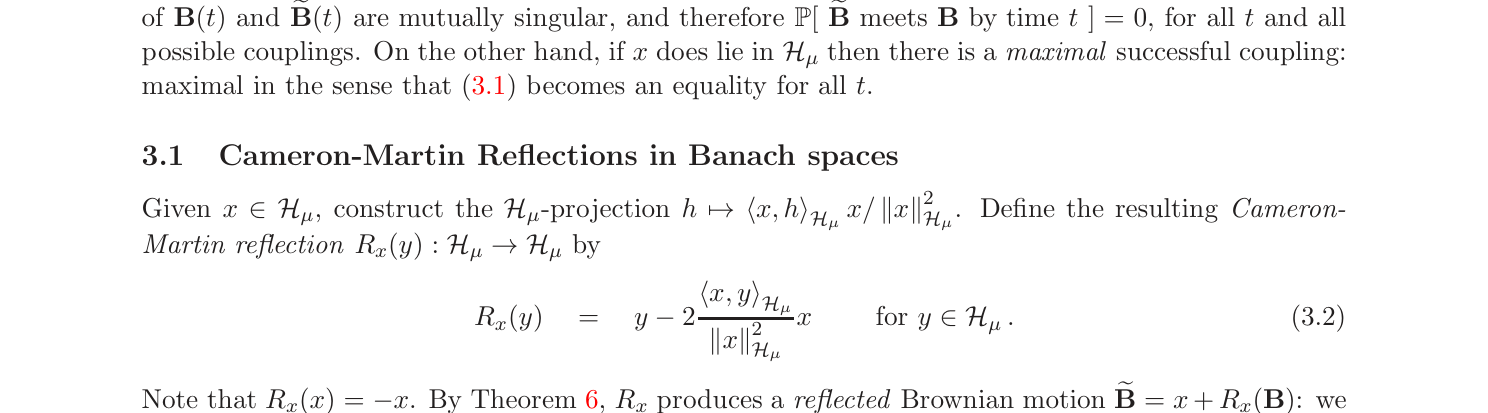
\includegraphics[width=\linewidth]{figures/reflection_definition_crop.png}
\end{center}

\section{Proof intuition}

The obstruction to finite-time coupling is that the initial displacement may
not lie in \(\HH\).  But \(\HH\) is dense in \(\W\).  We therefore write the
displacement \(x\in\W\) as a convergent telescoping sum of Cameron--Martin
corrections \(h_n\in\HH\), with
\[
        x=h_1+h_2+\cdots
        \quad\text{in }\W
\]
and with \(\sum_n \norm{h_n}_{\W}<\infty\).  At stage \(n\), the two Brownian
motions differ by a deterministic residual \(r_{n-1}=h_n+r_n\).  A reflection
coupling in the single Cameron--Martin direction \(h_n\) removes \(h_n\) in
finite time, leaving the smaller deterministic residual \(r_n\).  Then the
motions are run synchronously for one unit of time, and the next stage begins.

The reflected stage can overshoot in the negative \(h_n\)-direction before it
hits the coupling hyperplane.  Its maximum scalar stretch has a heavy
one-dimensional gambler's-ruin tail, but when multiplied by the summable
\(\W\)-norms \(\norm{h_n}_{\W}\), Borel--Cantelli forces the stage suprema to
tend to zero.  Thus the Banach-space distance between the two paths tends to
zero along all times, not merely at stage endpoints.

\section{The theorem}

\begin{theorem}
Let \((\W,\HH,\mu)\) be an abstract Wiener space, with \(\HH\) densely and
continuously embedded in the separable Banach space \(\W\).  Let \(B\) be a
\(\W\)-valued Brownian motion whose time-one law is \(\mu\).  For any two
starting points \(a,b\in\W\), there is a coupling of \(\W\)-valued Brownian
motions \(B^a,\widetilde B^b\), started respectively at \(a\) and \(b\), such
that
\[
        \Prob\left[
        \norm{\widetilde B^b(t)-B^a(t)}_{\W}\to0
        \text{ as }t\to\infty
        \right]=1 .
\]
Consequently Question 18 of \cite{CandelleroKendall2017} has an affirmative
answer.
\end{theorem}

\begin{proof}
By translation invariance it suffices to start one Brownian motion at \(0\)
and the other at \(x=b-a\in\W\).  If \(x=0\), take the synchronous coupling.
Assume \(x\ne0\).

\subsection*{Step 1: a summable Cameron--Martin approximation}

Choose a positive summable sequence \((\varepsilon_n)_{n\ge1}\) tending to
zero, for instance \(\varepsilon_n=2^{-n}\).  Set \(r_0=x\).  Since \(\HH\)
is dense in \(\W\), choose inductively \(h_n\in\HH\) such that
\[
        r_n:=r_{n-1}-h_n,\qquad
        \norm{r_n}_{\W}\le \varepsilon_n .
\]
Then \(r_n\to0\) in \(\W\), and
\[
        r_{n-1}=h_n+r_n .
\]
Moreover, for \(n\ge2\),
\[
        \norm{h_n}_{\W}
        \le \norm{r_{n-1}}_{\W}+\norm{r_n}_{\W}
        \le \varepsilon_{n-1}+\varepsilon_n .
\]
Thus
\[
        \sum_{n=1}^\infty \norm{h_n}_{\W}<\infty .
\]

\subsection*{Step 2: one reflected reduction}

We record the elementary one-step coupling estimate.  Fix deterministic
\(r\in\W\) and \(h\in\HH\setminus\{0\}\).  Suppose at some stopping time the
two processes differ by \(r+h\).  From that time onward, use the
Cameron--Martin reflection coupling in the direction \(h\) until the
one-dimensional component hits the coupling hyperplane, and then run the
processes synchronously.  During the reflected part of this stage the
difference has the form
\[
        r+\alpha(t)h ,
\]
where \(\alpha(0)=1\), \(\alpha(t)>0\) before the hitting time, and
\(\alpha=0\) after it.  The hitting time is finite almost surely because it
is the hitting time of a real Brownian motion.

Let
\[
        A_h=\sup\{\alpha(t):\text{during this reflected stage}\}.
\]
Then for every \(M\ge1\),
\[
        \Prob[A_h\ge M]\le \frac1M .       \tag{1}
\]
Indeed, write \(\beta\) for the one-dimensional Brownian component in the
direction \(h/\norm{h}_{\HH}\), begun at \(0\), and stop it on first hitting
\(\norm{h}_{\HH}/2\).  Before this hit,
\[
        \alpha(t)=1-\frac{2\beta(t)}{\norm{h}_{\HH}} .
\]
Thus \(\{A_h\ge M\}\) is the event that \(\beta\) hits
\(- (M-1)\norm{h}_{\HH}/2\) before it hits \(+\norm{h}_{\HH}/2\).  The usual
gambler's-ruin formula for one-dimensional Brownian motion gives probability
\[
        \frac{\norm{h}_{\HH}/2}
        {(M-1)\norm{h}_{\HH}/2+\norm{h}_{\HH}/2}
        =\frac1M .
\]

\subsection*{Step 3: concatenate the stages}

Construct the pair stage by stage.  At the beginning of stage \(n\), arrange
that the deterministic difference is \(r_{n-1}=h_n+r_n\).  If \(h_n=0\), skip
the reflected part.  Otherwise, apply the one-step reflected reduction to
remove \(h_n\), leaving difference \(r_n\).  Then run the two paths
synchronously for one deterministic unit of time before beginning stage
\(n+1\).

Let \(\sigma_n\) be the end time of stage \(n\), including the one-unit
synchronous wait.  Since \(\sigma_n\ge n\), only finitely many stages occur
before any fixed deterministic time, and \(\sigma_n\to\infty\).

Each finite initial segment is a finite concatenation, at stopping times, of
ordinary Cameron--Martin reflection couplings and synchronous couplings.  By
the strong Markov property and the usual invariance of Brownian motion under
predictable orthogonal Cameron--Martin reflections, both marginals are
\(\W\)-valued Brownian motions.  Equivalently, for every finite family
\(\ell_1,\ldots,\ell_m\in\W^*\), the corresponding transformed coordinate
process is a continuous local martingale with covariance matrix
\[
        t\,
        \big(\operatorname{Cov}_\mu(\ell_i,\ell_j)\big)_{i,j=1}^m ,
\]
because the integrand is orthogonal on \(\HH\) at every time; Levy's
characterization gives the required finite-dimensional Brownian projections.
The path itself is \(\W\)-continuous, since on each finite time interval it is
obtained from the original \(\W\)-Brownian path by finitely many standard
reflections of the form used in \cite{CandelleroKendall2017}.

\subsection*{Step 4: convergence at time infinity}

Let \(A_n\) be the scalar stage supremum from Step 2 for the \(n\)-th
reflection, with \(A_n=0\) if \(h_n=0\).  During the reflected part of stage
\(n\),
\[
        \norm{\widetilde B(t)-B(t)}_{\W}
        \le \norm{r_n}_{\W}+ A_n\norm{h_n}_{\W},
\]
and during the following synchronous wait the distance is exactly
\(\norm{r_n}_{\W}\).

Fix \(\eta>0\).  For all sufficiently large \(n\), \(\norm{h_n}_{\W}<\eta\).
Using (1),
\[
        \Prob\!\left[
        A_n\norm{h_n}_{\W}>\eta
        \right]
        =
        \Prob\!\left[
        A_n>\frac{\eta}{\norm{h_n}_{\W}}
        \right]
        \le
        \frac{\norm{h_n}_{\W}}{\eta}.
\]
The right-hand side is summable in \(n\).  By Borel--Cantelli,
\[
        A_n\norm{h_n}_{\W}\longrightarrow0
        \qquad\text{almost surely.}
\]
Since also \(\norm{r_n}_{\W}\le\varepsilon_n\to0\), the supremum of
\(\norm{\widetilde B(t)-B(t)}_{\W}\) over all times in stage \(n\) tends to
zero almost surely.  Because the stage end times tend to infinity, this is
exactly
\[
        \norm{\widetilde B(t)-B(t)}_{\W}\to0
        \qquad\text{almost surely as }t\to\infty .
\]
This proves the theorem.
\end{proof}

\section{Verification and limitations}

The proof does not use a Schauder basis, FDD, or M-basis.  The only structural
input beyond the standard Banach-valued Brownian-motion framework is the
dense continuous embedding \(\HH\hookrightarrow\W\), which is part of the
abstract Wiener space setup and is stated in the source paper.

The important technical point for human review is the marginal-preservation
step in the infinite stage construction.  Since a deterministic one-unit
synchronous wait follows every reflected stage, only finitely many reflections
occur on any bounded time interval.  Thus no finite-time definition involves
an infinite product of reflections.  The proof reduces the marginal law on
each bounded interval to the standard Cameron--Martin reflection coupling
used by the source paper, concatenated at stopping times.

The convergence estimate deliberately avoids moments of \(A_n\), whose
expectation is infinite.  It uses only the tail bound
\(\Prob[A_n\ge M]\le M^{-1}\) and the summability of
\(\norm{h_n}_{\W}\).

\section{Novelty check}

Before promotion, I searched the run indexes
\[
\texttt{registry\_index.tsv},\quad
\texttt{solutions/index.tsv},\quad
\texttt{attempts/index.tsv},\quad
\texttt{proof\_gaps/index.tsv}
\]
for the arXiv id, title, and core phrases including
\texttt{coupling at time infinity}, \texttt{abstract Wiener space}, and
\texttt{Brownian coupling}.  No existing packet or attempt answered this
target.

I also searched the local parsed source corpus for the exact coupling phrases
and close abstract-Wiener keywords.  The only relevant occurrences were the
source paper and target-pool metadata.  A bounded web search using the queries
\[
\begin{gathered}
\texttt{"coupling at time infinity" "abstract Wiener space"},\\
\texttt{"Brownian coupling at time infinity" "Banach"},\\
\texttt{"Coupling of Brownian motions in Banach spaces" "open question"},\\
\texttt{"Cameron-Martin" "coupling at time infinity" Brownian}
\end{gathered}
\]
and close variants found only the source arXiv page as a relevant hit.  This
is therefore recorded as a candidate original proof, not as an established
literature answer.  Novelty confidence remains bounded-search confidence,
pending specialist review.

\section{Human review recommendation}

Review as a high-priority candidate full solution to Question 18.  The proof
is short and appears to bypass the basis machinery in the source paper by
turning the paper's \(\varepsilon\)-approximate coupling remark into an
iterated construction.  A reviewer should focus first on whether predictable
concatenations of Cameron--Martin reflections in changing deterministic
directions preserve the second process as a Banach-valued Brownian motion.
If that step is accepted, the remaining approximation and Borel--Cantelli
argument is elementary.

\begin{thebibliography}{9}

\bibitem{CandelleroKendall2017}
E. Candellero and W. S. Kendall,
\emph{Coupling of Brownian motions in Banach spaces},
arXiv:1705.08300, 2017.
\url{https://arxiv.org/abs/1705.08300}.

\end{thebibliography}

\end{document}
